\subsubsection{ABN-Encoder}
\label{subsubsec:Inbetriebnahme_ABN-Encoder}

Der ABN-Encoder wird mit einem Testprogramm in Betrieb genommen. Das Programm initialisiert die benötigte Hardware des Mikrocontrollers (UART, SPI, Pins), enthält die Library des FOC- und Gate-Treibers und ermöglicht das Debugen über die serielle Schnittstelle. Da der ABN-Encoder am FOC-Treiber angeschlossen ist, wird die Schnittstelle für den ABN-Encoder am FOC-Treiber initialisiert. Dazu müssen weitere Register gesetzt werden, worunter auch die Register für die PI-Regler fallen. Die Software TMCL-IDE hilft bei der Bestimmung der Parameter für den ABN-Encoder und PI-Regler. Welche Register wie beschrieben wurden ist im Anhang Kapitel \ref{Appendix:ABN_Register} zu sehen. Die Initialisierung sowie das Auslesen gewisser Register ist mit der Testapplikation ''\textit{4\underline{ }Motor\underline{ }ABN\underline{ }Encoder}'' möglich.

Es wird erwartet, dass der FOC-Treiber im Positionsmodus im ersten Moment stehen bleibt. Wird jetzt der Rotor gedreht, muss der FOC-Treiber die Abweichung nachkorrigieren. Wird dem Motor eine andere Position vorgegeben, muss der Motor sich an die gewünschte Position fahren und dort halten.

Die Werte der PI-Regler wurden Experimentell bestimmt. Folgende Werte wurden dabei ermittelt:

\begin{tabularx}{\linewidth}{|l|X|X|l|}
\hline
\textbf{Regelkreis} & \textbf{P-Anteil} & \textbf{I-Anteil} & \textbf{Nachstellzeit}\\
\hline
Drehmoment & 100 & 1200 & \\
\hline
Fluss & 100 & 1200 & \\
\hline
Geschwindigkeit & 2000 & 300 & \\
\hline
Position & 100 & 0 & \\
\hline
\end{tabularx}

\todo{Nachstellzeit?}

Die Limits wurden folgendermassen gesetzt:

\begin{tabularx}{\linewidth}{|l|X||l|X|}
\hline
\textbf{Limit} & \textbf{Wert} & \textbf{Limit} & \textbf{Wert}\\
\hline
Drehmoment & 2500 & Fluss & 2500\\
\hline
Geschwindigkeit & 1500 &  & \\
\hline
\end{tabularx}

Die Regler wurden so bestimmt, dass die Regelkreise in unbelasteten Zustand ihre Sollwerte schnellst möglich erreichen, ohne überzuschiessen. Dies betrifft den Regler für den Stromregelkreis und den Regler für den Geschwindigkeitsregelkreis. Die zugehörigen Parameter wurden in der TMCL-IDE ermittelt. 

\begin{figure}[H]
	\centering
	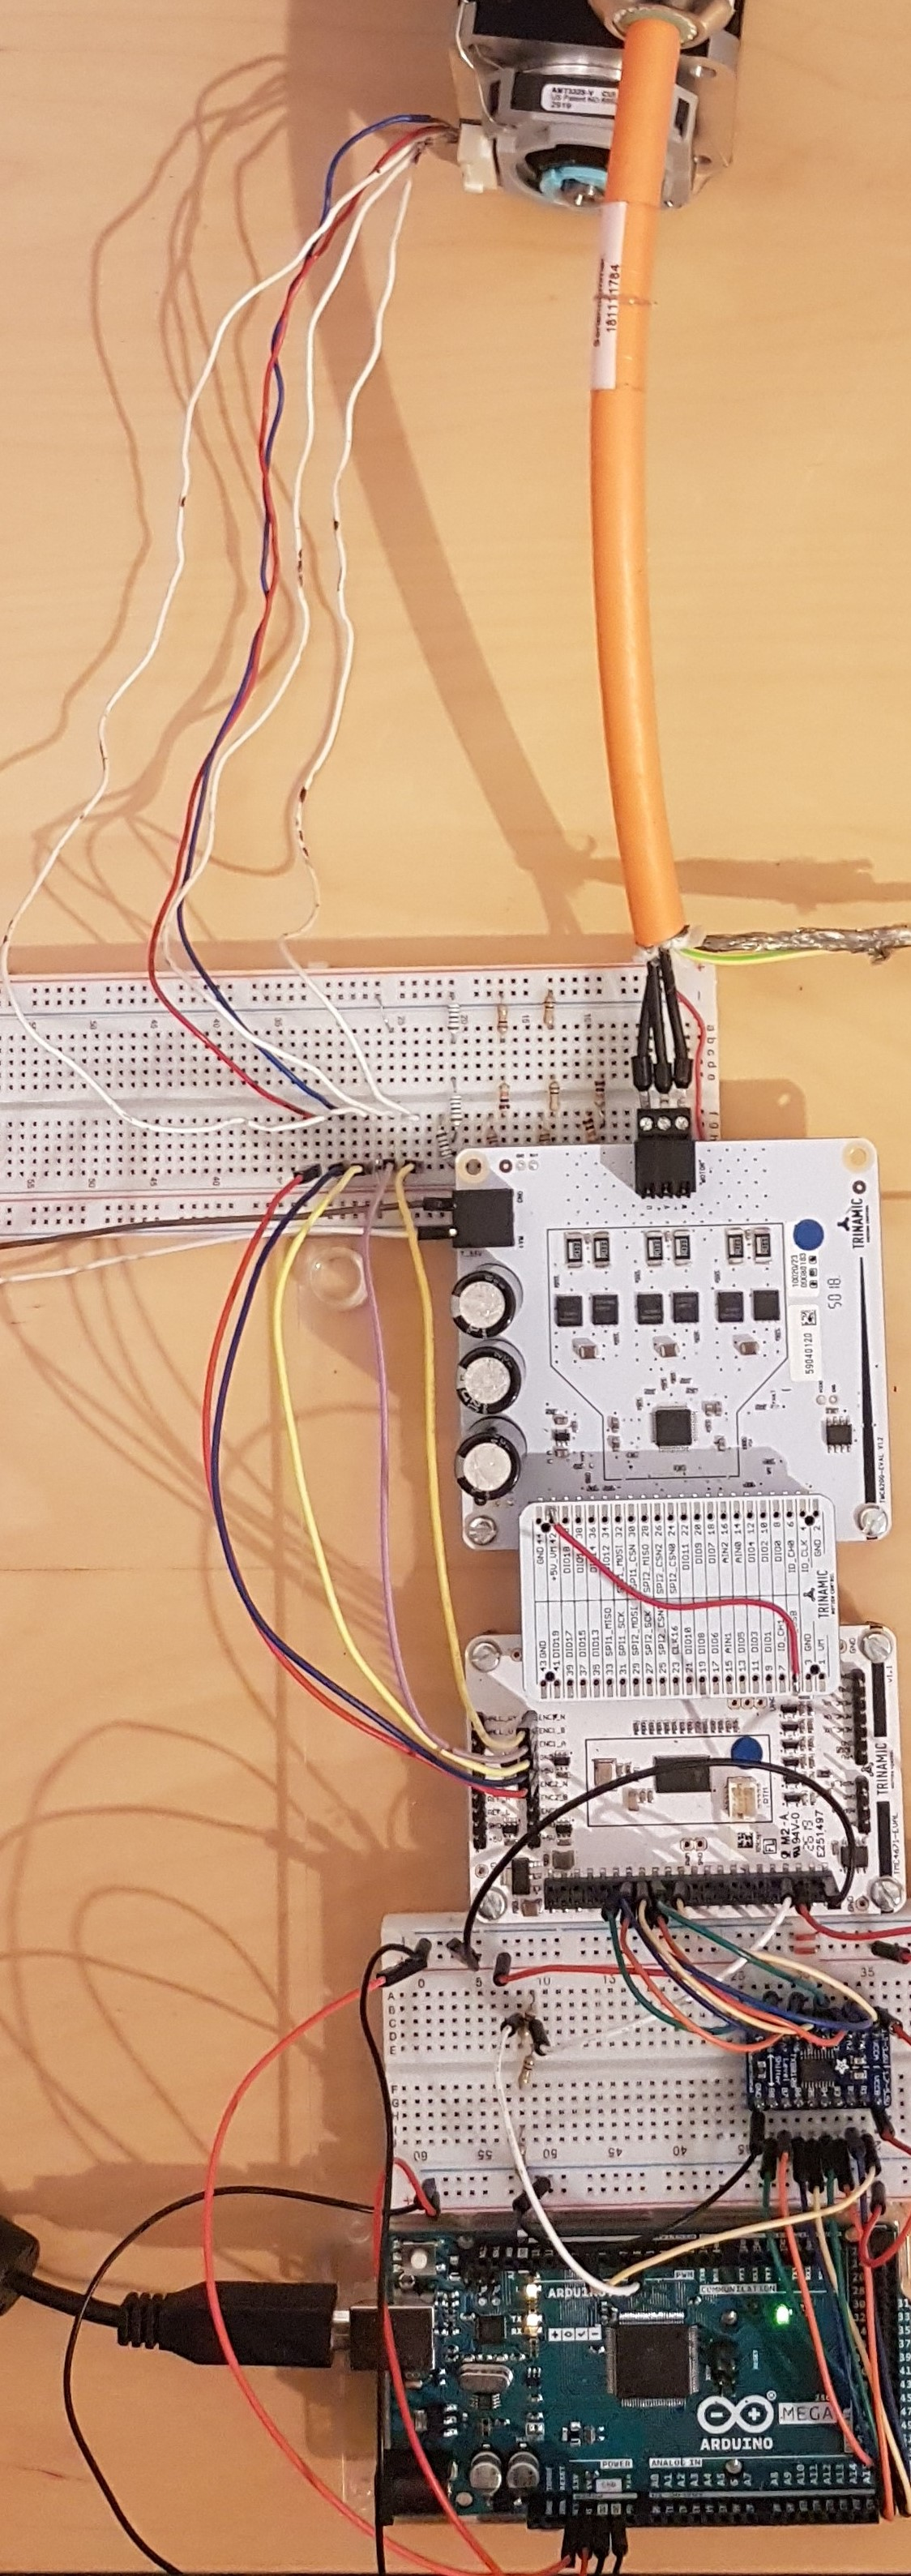
\includegraphics[angle = 270, width=\textwidth]{graphics/4_komplett}
	\caption{Komplettansicht mit Mikrocontroller, Level-Shifter, FOC-Treiber, Gate-Treiber, H-Brücke, ABN-Encoder und Motor.}
	\label{fig:4_komplett}
\end{figure}
\newpage
\textbf{Achtung}, wenn die Scripts auf den Mikrocontroller des PartyMixers geladen werden ist darauf zu achten, dass die Achse des Motors frei beweglich ist und das Förderband nicht mit der Achse mitdreht, da ansonsten Schäden an der Maschine entstehen können. Es wird empfohlen die Scripts mit Mikrocontroller und EVAL-Boards zu testen.

Vorgehen:
\begin{enumerate}
\item Benötigte Applikation, welche im Software-Ordner auf dem USB-Stick oder Github \cite{aebi_projekt-6softwareatmega_2020} zu finden ist, in Atmel Studio öffnen.\\
\textcolor{magenta}{Software\textrightarrow Atmega\textrightarrow 4\underline{ }Motor\underline{ }ABN\underline{ }Encoder\textrightarrow 1\underline{ }Motor\underline{ }Testsoftware\textrightarrow Motor}\\

\item Software hochladen:\\
\textcolor{blue}{AtmelStudio\textrightarrow Tools\textrightarrow PartyMixer}\\


\end{enumerate}

Ergebnis: Nach der Initialisierung wird zuerst ein Testdrive ausgeführt, welcher den Rotor mit hoher Geschwindigkeit eine Sekund nach links und eine Sekunde nach Rechts drehen lässt. Danach wird der Motor in den Positionsmodus versetzt, wordurch der FOC-Treiber bei einer Störung von ausserhalb nachkorrigiert, um wieder auf die Ursprungsposition zu kommen. Wird über den seriellen Monitor '1' eingegeben, fährt der Motor 12 verschiedene Positionen an und dann wieder zurück zur Ursprungsposition. Wird Enter gedrückt, wird die Position inkrementiert. Wird '0' gedrückt, fährt der Motor an die Ursprungsposition zurück.

Die Problematik besteht in der Kontrolle des Motors. So wie die Regler ausgelegt sind, kann der Schlitten, welcher vom Motor bewegt wird, nicht sorgfältig genug bewegt werden. Abhilfe schafft eine Software-Ramp, welche den Weg unter Vorgabe einer Höchstgeschwindigkeit und -Beschleunigung berechnet. Die Ramp gibt dem FOC-Treiber schrittweise die Positionen vor, wodurch dur Motor für den Bruchteil einer Sekunde wartet, bis die nächste Position vorgegeben wird.